% include the figures path relative to the master file
% \graphicspath{ {./content/method/figures/visual_cues/}{./content/method/figures/}}
\graphicspath{ {./content/method/figures/}}

\begin{figure}[t]
  \centering{
    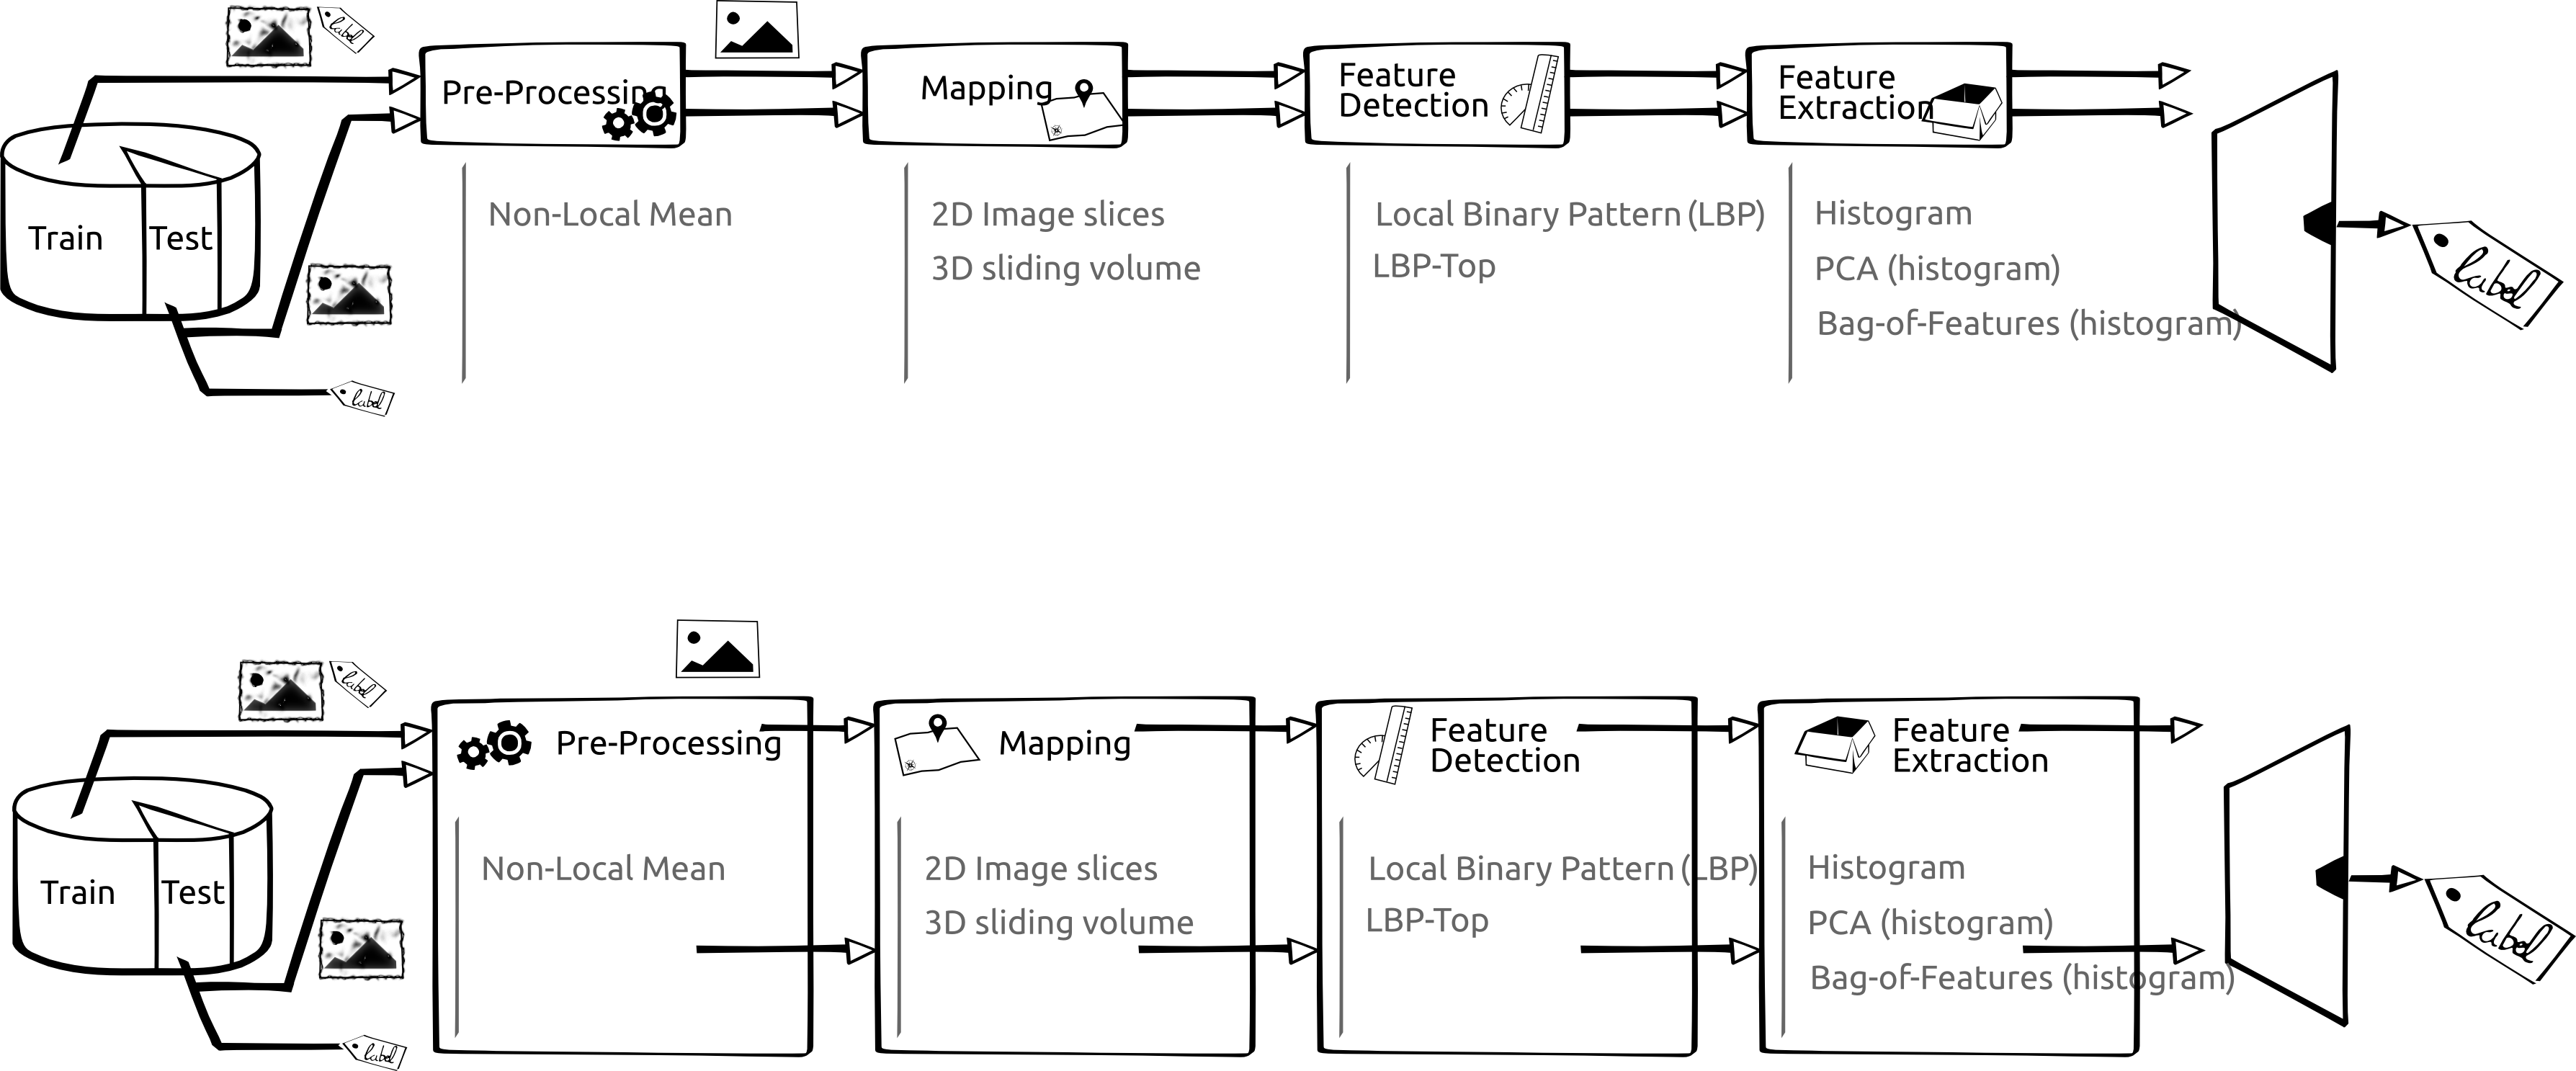
\includegraphics[width=1\textwidth]{ml}}
  \caption{Machine learning classification basic scheme}
  \label{fig:ML-scheme}
\end{figure}

\section{Materials and Methods}\label{sec:method}

The proposed method, as well as, its experimental set-up for \ac{oct} volume classification are outlined in Fig.\,\ref{fig:ML-scheme}.
The methodology is formulated as a standard classification procedure.
% The available dataset with its acompaining \ac{gt} are divided into training $(S1,l1)$ and testing $(S2,l2)$. 
% The final goal is to represent $S1$ and $S2$ in the feature space $F$ by supplying $(sxF,l1)$ as a training to a classifier, using the trained classifier to estimate $l2$ from $S2xF$ and comparing the estimation with the \ac{gt}.
First, the \ac{oct} volumes are pre-processed as presented in details in Sect.\,\ref{subsec:prepro}.
% This algorithm preserve important details and textures of the original image, while reducing the noise.
The mapping stage is used to determine a discrete set of elements (or structures) which is used for representing the \ac{oct} volume.
Thereafter, two mapping strategies are defined: (i) \emph{global} and (ii) \emph{local} mapping.
In the global mapping approach, a single structure is computed for the image/volume while in the local mapping, a set of structures is defined by sliding a window through the image/volume.
Then, a descriptor is computed for each structure.
The feature extraction and representation are presented in depth in Sect.\,\ref{subsec:feaext} and Sect.\,\ref{subsec:fearep}.
% The feature detection stage correspond to measurements done in $G(Z)$ used for representing $s$ in terms of $ZxG$. 
% This mapping and feature detection steps can be found as a single-steps in the literature.
% The feature extraction procedure combines the elements in $Z$ and its measurements $G(Z)$ to create the final feature space $F$ and project $s$ on it.
A \ac{rf} classifier has been selected to perform the classification of the \ac{oct} volume~\cite{breiman2001random}.
% The design choices are all illustrated in Fig.\,\ref{fig:ML-scheme} and discussed further in this section. The work here presented does not discuss in detail neither the mapping, nor the adopted classifier, further than this lines.
% As a possible mappings, for representing the volumes, 2D image slices of the volume and \color{red}{7x7x7}\color{black} sliding volumes, have been considered. 
% As a classifier, a \color{red}{Random Forest}\color{black} using 100 trees, has been considered.

% \subsection{Data}
% \color{red}{
%   \begin{itemize}
%   \item cross-validation
%   \item our dataset
%   \item DUC dataset
%   \end{itemize}}\color{black}

% For evaluation purposes, the results have been cross-validated, by splitting the data in training and testing using a \ac{lopo} strategy. In this manner for each round a pair \color{red}{dce,normal} has been selected to be used as the round test set, while the rest of the dataset has been used as a training. \color{red}{Doing the cross validation in this manner, has the limitation that despite the fact that the results are robust due to the cross validation, no results variance can be reported. However, and despite this limitation, \ac{lopo} has been choose due to the reduced amount of \ac{oct} volumes available.}\color{black}

% \color{red}{The dataset blablablabal...}\color{black}
% \color{red}{The duc dataset blabla bla...}\color{black}

\subsection{Image pre-processing}\label{subsec:prepro}

\Ac{oct} images are known to be affected by a speckle noise~\cite{schmitt1999speckle}.
Subsequently, \ac{nlm}~\cite{buades2005non} filtering has been successfully used in \ac{us} images to filter similar noise~\cite{Coupe2009} and is used in our framework to denoise each B-scan (i.e. each $x-z$ slice) of the \ac{oct} volumes (see in Fig.\,\ref{subfig:vol}).
%The pre-processing stage in the proposed methodology applies an image denoising method to reduce the speckle noise in \ac{oct} images.
%Since image details and texture of the original image are needed by the following stages in the method, \ac{nlm} algorithm \cite{buades2005non} is used. 
\ac{nlm} filtering offers the advantage to use all the possible self-predictions that the image can provide rather than local or frequency filters such as Gaussian, anisotropic or Wiener filters~\cite{buades2005non}.
An example of filtering using \ac{nlm} filter on \ac{oct} image is depicted in Fig\,\ref{subfig:raw} and Fig.\,\ref{subfig:nlm}.

\begin{figure}[t]
  \centering
  \hspace*{\fill}
  \subfigure[]{\label{subfig:vol}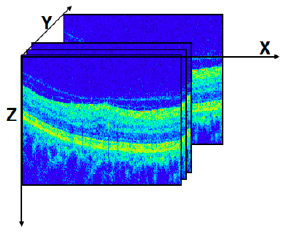
\includegraphics[width=0.3\linewidth]{volume.png}} \hfill
  \subfigure[]{\label{subfig:raw}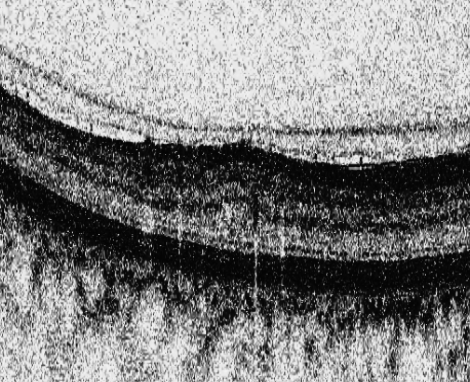
\includegraphics[width=0.3\linewidth]{raw_crop_grey.png}} \hfill
  \subfigure[]{\label{subfig:nlm}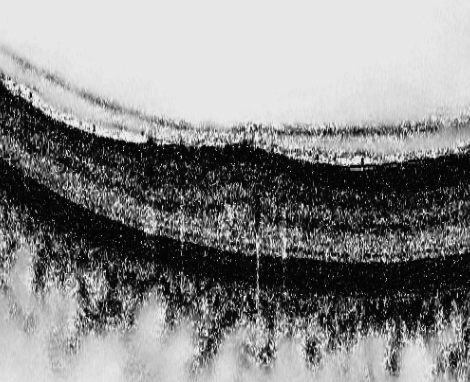
\includegraphics[width=0.3\linewidth]{nlm_crop_grey.png}}
  \hspace*{\fill}
  \caption{\ac{oct}: (a) Organization of the \ac{oct} data - (b) Original image - (c) \ac{nlm} filtering.}
  \label{fig:denoise}
\end{figure}

\subsection{Features extraction}\label{subsec:feaext}

\ac{lbp} is a texture descriptor based on the signs of the differences of a central pixel with respect to its neighboring pixels~\cite{ojala2002multiresolution}. 
%More precisely, this descriptor encodes the intensity differences of a central pixel ($g_c$) with its neighboring pixels ($g_{p}$), within in a defined neighborhood of radius $R$. 
These differences are encoded in terms of binary patterns as in~Eq.\,\eqref{Eq:LBP}: 

\begin{equation}\label{Eq:LBP}
LBP_{P,R} = \sum_{p=0}^{P-1}s(g_{p} - g_{c})2^{p} \ , \qquad s(\cdot) = \begin{cases}
    1  & \ \text{if } (g_{p} - g_{c}) \geq 0\\
    0  & \ \text{otherwise}\\
  \end{cases} \ ,
\end{equation}

% \begin{align} \label{Eq:LBP}
% LBP_{P,R} = \sum_{p=0}^{P-1}s(g_{p} - g_{c})2^{p}& \ , \\
% \text{where } &s(\cdot) = \begin{cases}
%     1  & \quad \text{if } g_{p} - g_{c} \geq 0\\
%     0  & \quad \text{otherwise}\nonumber\\
%   \end{cases} \ .
% \end{align}
\noindent where $g_c$, $g_{p}$ are the intensities of the central pixel and a given neighbor pixel, respectively. $P$ is the number of sampling points in the circle of radius $R$. Figure~\ref{subfig:lbp} illustrates the meaning of $P$ and $R$.

Ojala\,\textit{et al.} further extend the original \ac{lbp} formulation to achieve rotation invariance at the expense of limiting the texture description to the notion of circular ``uniformity''~\cite{ojala2002multiresolution}. Volume encoding is later proposed by Zhao\,\textit{et al.} by computing \ac{lbp} descriptors in each orthogonal planes, so called \ac{lbptop}~\cite{zhao2012rotation}.

\begin{figure}[t]
  \centering
  \hspace*{\fill}
  \subfigure[]{\label{subfig:lbp}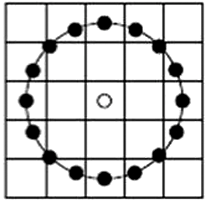
\includegraphics[height=0.15\textheight]{lbp.png}} \hfill
  \subfigure[]{\label{subfig:lbptop}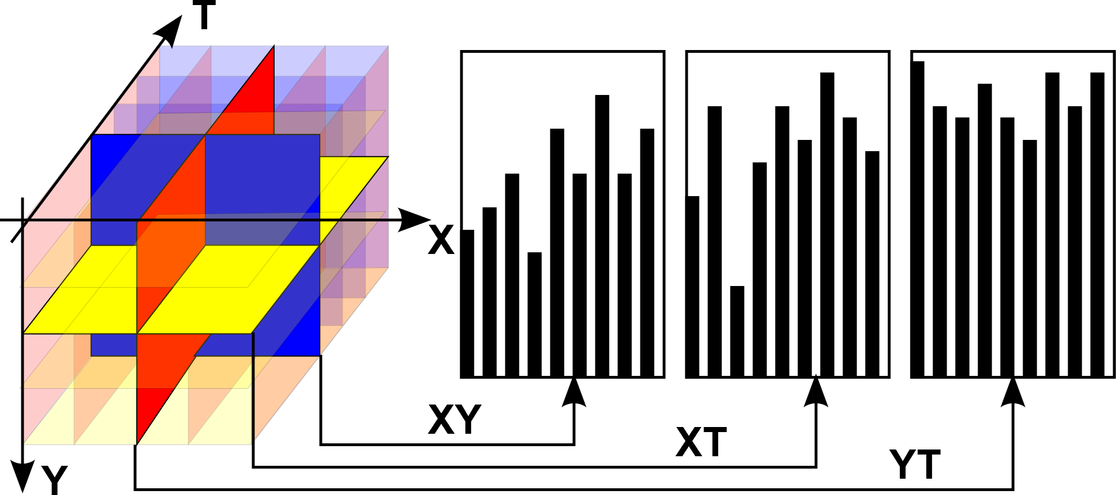
\includegraphics[height=0.15\textheight]{LBPTOP_fig.png}}
  \hspace*{\fill}
  \caption{The different \ac{lbp} descriptors: (a) \ac{lbp} with $(R=2,P=16)$ - (b) \ac{lbptop}~\cite{zhao2012rotation}.}
  \label{fig:lbp}
\end{figure}

\subsection{Feature representation}\label{subsec:fearep}

Each \ac{oct} volume can be described by its texture and we employed two strategies.

\begin{description}

\item[Low-level representation] The texture descriptor of an \ac{oct} volume is defined as the concatenation of the \ac{lbp} histograms. Regarding the \ac{lbptop}, the feature descriptor is computed through the concatenation of the \ac{lbp} histograms of the three orthogonal planes. 
Furthermore, the size of this entire feature vector is defined according to the mapping strategy chosen (see Fig.\,\ref{fig:ML-scheme}).

\item[High-level representation] According to the chosen mapping strategy, the low-level representation can lead to a high dimensional feature space. 
High-level representation simplifies this high dimensional feature space into a more discriminant lower space. 
\Ac{pca} and \ac{bow} among other methods, are used for this purpose~\cite{Sivic2003}. 
Although \ac{pca} maps the data according to their variance, \ac{bow} models represent the features by creating a visual dictionary, or ``codebook'', from the set of low-level features.
The set of low-level features is clustered using \textit{k}-means to create the codebook with \textit{k} defining the number of visual words.
After creating the codebook, each of the training example is represented as a histogram of size \textit{k} obtained by calculating the frequency of occurrences of each of the \textit{k} words in the features extracted from the training example. 

\end{description}

%\subsubsection{Low-level features} are extracted considering the whole volume using LBP and 3D-LBP descriptors. 
% LBP is a discriminative rotation invariant feature descriptor proposed by Ojala et al. \cite{ojala2002multiresolution}. 
% LBP descriptor encodes the intensity differences of a central pixel ($g_c$) with its neighboring pixels ($g_{p}$), within in a defined neighborhood of radius $R$. The differences are encoded in terms of binary patterns as in~Eq. \ref{Eq:LBP}: 

% \begin{equation} \label{Eq:LBP}
% LBP_{P,R} = \sum_{p=0}^{P-1}s(g_{p} - g_{c})2^{p},
% \end{equation}
% where $s(a) = 1$ if $a \geq 0$, and $s(a)=0$ otherwise. $P$ is the number of sampling points in the circle of radius $R$.

% The binary patterns are calculated for each pixel in the given image and their histogram defines the final descriptor.
% The LBP histograms are computed for each slice of the volume and are concatenated into a single histogram. This forms the first low-level feature.
% The second low-level descriptor is defined in a similar manner as the first one. However principal component analysis (PCA) is applied to the concatenated histograms in order to reduce the dimension.

% For the third low-level descriptor, since the OCT data is a 3D volume, following the approach of Zhao \textit{et al}. \cite{zhao2007dynamic}, we extract 3D-LBP by considering three orthogonal planes, XY, XZ and YZ. Note that $X$, $Y$, and $Z$ are respectively the horizontal, vertical and depth direction of the OCT volume as shown in Figure~\ref{fig:oct_data}(a).
% LBP patterns are computed for each of the three planes, and the obtained three histograms are concatenated into a final 3D-LBP descriptor.



% \subsubsection{High-level features} - are extracted using bag of words (BoW) approach which is a feature representation technique based of creating a visual dictionary, or codebook, from a set of low-level features~\cite{Sivic2003}. 
% To do so, the OCT images are divided into local patches and LBP histograms are computed for every local patch.
% This set of LBP histograms is then used to create a codebook using K-means clustering. If we define $K$ clusters in the feature space, then the visual dictionary will contain $K$ words each one being the center of one cluster.
% After creating the codebook, each of the training example is represented as a histogram of size $K$ obtained by calculating the frequency of occurrences of each of the $K$ words in the features extracted from the training example. 
% Note that in the 2D case, each slice is divided into patches of size $N\times N$ and we extract 2D-LBP from each patch, while in the 3D case, the volume is divided into $N \times N \times N$ patches and 3D-LBP histograms are computed. In our experiments in Section 3, we set $N=7$, and vary the size of the codebook $K$ in the range $\{2, 4, 8, 16, 32, 64, 100 \}$.
% % \tikzstyle{block} = [rectangle, draw, fill=gray!20, text = black,
    text width=6em, text centered, rounded corners, minimum height=4em , minimum width = 6em]
    % \tikzstyle{line} = [draw, -latex']
  \tikzstyle{myarrow}=[->, thick]
    \tikzstyle{line}=[-, thick]
    \tikzstyle{block2} = [rectangle, draw, fill=white!20,
    text width=6em, text centered, rounded corners, minimum height=4em, minimum width = 6em]
    \tikzstyle{block3} = [rectangle, draw, fill=gray!20, text = black,
    text width=7em, text centered, rounded corners, minimum height=4em , minimum width = 7em]
\def\blockdist{1}
\def\edgedist{1.5}
  %%%% The Framework Sparse Coding 

\begin{figure}
 \begin{center}
   \begin{tikzpicture}[node distance = 1cm,scale=0.6, every node/.style={scale=0.6}]
%(FEx.east|- FEx.south)
    \node [block2] (input) {Training image};
    %\node [block, right of = input, node distance = 2.8cm](Seg){Segmentation}; 
    \node [block, right of=input,node distance = 2.8cm](De){Denoising};
    \node [block, right of=De,node distance = 2.8cm](FEx){Feature extraction};
    \path (FEx.east)+(+0.8,0) node (g) {};
    
    %%% Sparse Coding Block
    \node [block3, right of=g,node distance = 1.7cm](DL){Dictionary learning /k-means};
    \node [block3, below of=DL,node distance = 2.5cm](PR){Projection};
    \begin{pgfonlayer}{background}
      \path (DL.west |- DL.north)+(-0.4,-0.1+\blockdist) node (a) {};
      \path (PR.east |- PR.south)+(+0.4,-0.7) node (b) {};          
      \path[fill=gray!10,rounded corners, draw=gray!20, dashed] (a) rectangle (b);
    \end{pgfonlayer}
\path (DL.west |- DL.north)+(+1.2,-0.5+\blockdist) node (SP) {\textbf{Bag of Features}};
\path (PR.east |- PR.south)+(-1.3,-0.4+\blockdist) node (c){};
\path (PR.east)+(-3.15,0) node (d) {};

%%% Testing 
\node [block, below of=FEx, node distance = 2.5cm](FE2){Feature extraction};
\node [block, below of=De, node distance = 2.5cm](De2){Denoising};
% \node [block, below of=Seg, node distance = 2.5cm](Seg2){Segmentation}; 
\node [block2, below of=input, node distance = 2.5cm](TestImg){Testing image};

%%% 
\node [block, right of=PR, node distance = 3.6cm](Pool){Visual words histogram};
\path (Pool.east) + (0.3,0) node (f){}; 
\path (Pool.east) + (0.2,-0.1) node (f1){}; 

%%% Classification
\node [block, right of = Pool, node distance = 3.5cm] (Pre){Prediction}; 
    \node [block, above of = Pre, node distance = 2.5cm] (Learn){Learning}; 
    \begin{pgfonlayer}{background}
      \path (Learn.west |- Learn.north)+(-0.4,-0.1+\blockdist) node (h) {};
    \path (Pre.east |- Pre.south)+(+0.4,-0.7) node (i) {};          
    \path[fill=gray!10,rounded corners, draw=gray!20, dashed] (h) rectangle (i);
\end{pgfonlayer}
\path (Learn.west |- Learn.north)+(+1.1,-0.5+\blockdist) node (Clas) {\textbf{Classification}};
\path (Pre.east |- Pre.south)+(-1.3,-0.4+\blockdist) node (j){};
\path (f1.north)+(0, 2.5) node (k) {};
\path (Pre.east) + (1.2,0) node (k1) {P(..)}; 

    % Draw edges
    \draw [line] (input) -- (De) -- (FEx); 
    \draw [myarrow] (FEx)-- (DL);
    \draw [myarrow] (DL) -- (PR) ; 
    \draw [line] (TestImg) -- (De2) -- (FE2); 
    \draw [myarrow] (FE2) -- (PR) ;
    \draw [line] (PR) -- (Pool); 
    \draw [myarrow] (Pool) -- (Pre); 
    \draw [line] (f1.north) -- + (0,2.5)(k.south); 
    \draw [myarrow] (k.south)+ (0,0.1)  -- (Learn.west); 
    \draw [myarrow] (Pre) -- (k1);

    \end{tikzpicture}
    \end{center}
    

\caption{Bag of features framework} 
\label{fig:BoF-framework}

\end{figure}

% \subsection{Classification}

% Random Forest is an ensemble of decision trees and was introduced by~\cite{breiman2001random}.
% The ensemble uses each tree to predict an output and finalize the ultimate prediction by aggregating the outputs of all tress. 
% This classifier learns the data by training multiple decision trees on bootstrap samples of the original data. 
% Each bootstrap of D dimension is used for training one decision tree and at each node, the best split among randomly ($d << D$) selected subset of descriptors is chosen. 
% Each tree is grown to its maximum length without any pruning. 
% In the prediction stage a sample is voted by each tree and it is labeled by considering the majority of the votes.


%%% Local Variables: 
%%% mode: latex
%%% TeX-master: "../../master"
%%% End: 
